\documentclass[a4paper,11pt]{article}
\usepackage[utf8]{inputenc}
\usepackage[T1]{fontenc}
\usepackage[margin=1in]{geometry}
\usepackage{graphicx}
\usepackage{booktabs}
\usepackage{array}
\usepackage{xcolor}
\usepackage{hyperref}
\usepackage{listings}
\setlength{\parindent}{0pt}
\setlength{\parskip}{0.6em}
\pagestyle{empty}
\lstset{basicstyle=\ttfamily\footnotesize,breaklines=true,breakatwhitespace=true,columns=fullflexible}
\begin{document}

\section*{Procedural Music Generator}

This repository contains a procedural music generator developed as part of a master's thesis at NTNU. The program generates tonal melodies from configurable musical settings and can also produce simple four-part harmonizations.

\begin{center}

  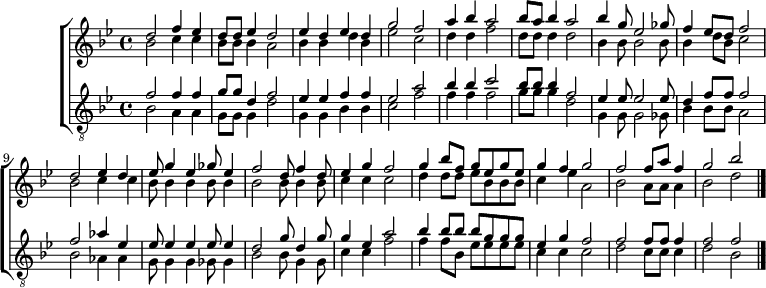
\includegraphics[width=0.95\linewidth]{../examples/iter3/iter3_long_explicit_chorale_bb.cropped.png}

\end{center}

\subsection*{Quick start}

\begin{lstlisting}[breaklines=true,breakatwhitespace=true,language=bash]

python3 code/main.py --form sentence --pdf --wav

\end{lstlisting}

This generates a melody with a sentence-like form and optionally renders notation and audio.

\subsection*{What the program does}

The current generator supports:

\begin{itemize}

  \item tonal melody generation in different keys and modes

  \item form-aware generation with \texttt{auto}, \texttt{sentence}, \texttt{period}, and \texttt{phrase}

  \item automatic or explicit harmonic plans

  \item rhythmic restriction through configurable allowed durations

  \item different voice profiles and ranges

  \item melody-only or chorale-style output

  \item LilyPond export, with optional PDF and WAV rendering

\end{itemize}

The system is built around an object-oriented music model and a weighted soft-constraint approach. In practice, this means the generator creates candidate melodies and prefers the ones that better satisfy musical rules such as stepwise motion, cadence shaping, chord-tone preference, and motivic reuse.

\subsection*{At a glance}

\begin{center}
\small
\begin{tabular}{p{0.28\linewidth} p{0.62\linewidth}}
\toprule
Area & Support \\
\midrule
Keys and modes & Major, minor, and modal tonal settings \\
Form & \texttt{auto}, \texttt{sentence}, \texttt{period}, \texttt{phrase} \\
Harmony & Automatic or explicit beat-based plans \\
Texture & Single melody or chorale-style output \\
Rendering & LilyPond source, cropped PDF, WAV \\
Control surface & CLI with reusable configuration in \texttt{code/main.py} \\
\bottomrule
\end{tabular}
\normalsize
\end{center}

\subsection*{Repository layout}

\begin{itemize}

  \item \texttt{code/} -- the music generator and CLI

  \item \texttt{docs/} -- user-facing program documentation

  \item \texttt{thesis/} -- thesis source, figures, and example material

  \item \texttt{webpage/} -- archive-page builder for generated thesis examples

\end{itemize}

\subsection*{Basic usage}

Run the generator from the repository root:

\begin{lstlisting}[breaklines=true,breakatwhitespace=true,language=bash]

python3 code/main.py

\end{lstlisting}

Common examples:

\begin{lstlisting}[breaklines=true,breakatwhitespace=true,language=bash]

python3 code/main.py --key D --mode major --bars 8 --seed 1337

python3 code/main.py --form sentence --pdf --wav

python3 code/main.py --texture chorale --key Eb --bars 8 --seed 2000 --pdf --wav

python3 code/main.py --harmony "2I,2V,4I,2IV,2iv" --seed 3000 --pdf

python3 code/main.py render --seed 1337 --pdf --wav

\end{lstlisting}

Generated LilyPond files are written to \texttt{code/output/\textless{}seed\textgreater{}/} by default. Optional rendering uses LilyPond for notation output and TiMidity++ for WAV export.

\subsection*{How it is structured}

\begin{itemize}

  \item \texttt{code/main.py} defines the default project configuration, especially the soft-constraint weights.

  \item \texttt{code/app\_cli.py} contains the reusable command-line workflow.

  \item \texttt{code/melody\_engine/} contains the musical data structures, generator logic, harmonization logic, and export pipeline.

\end{itemize}

This makes it possible to keep the CLI stable while still experimenting with different generator settings in \texttt{main.py}.

\subsection*{Documentation and thesis}

\begin{itemize}

  \item Program documentation: \texttt{docs/\_build/html/index.html}

  \item Thesis PDF: \texttt{thesis/latex/main.pdf}

\end{itemize}

Author-specific workflow notes for thesis building, archive generation, and deployment are kept in \texttt{thesis/README.md}.

\end{document}
